\newpage
\section{Abbilden Graphischer Objekte}

\subsection{Kameramodell}

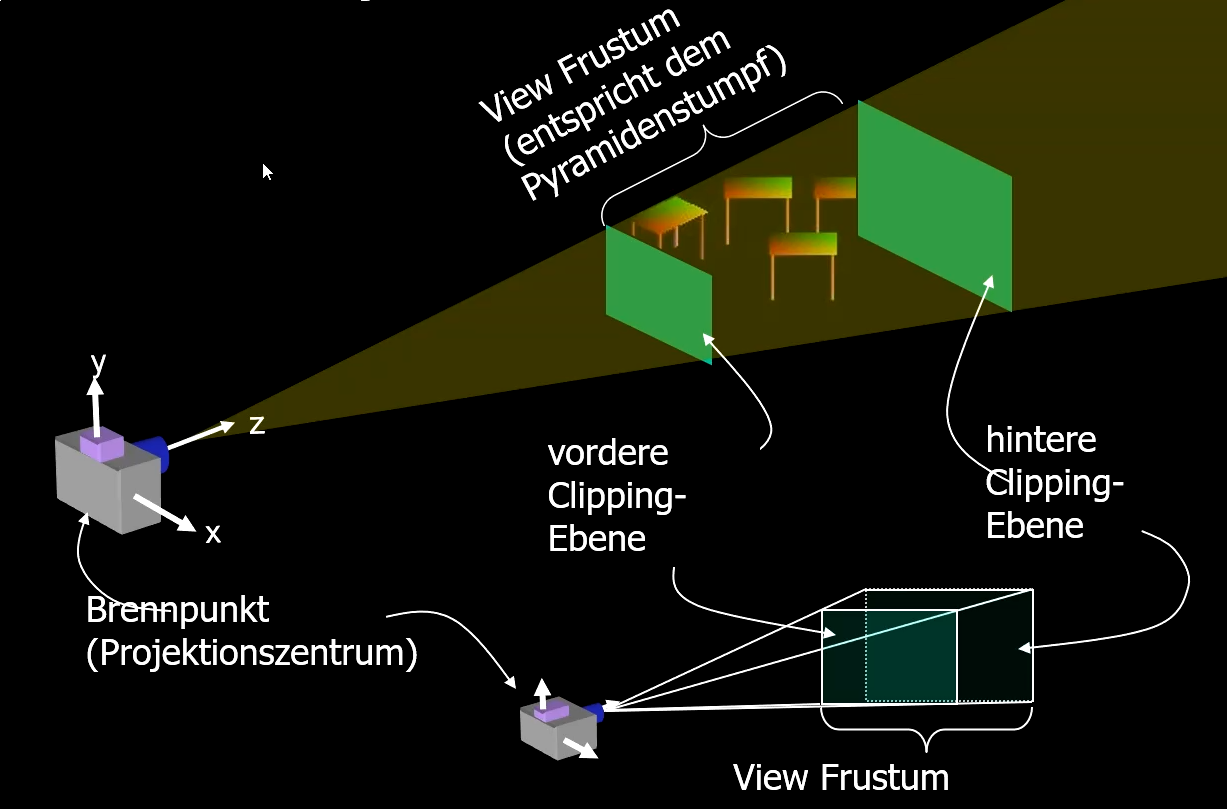
\includegraphics[width=400px]{images/kameramodell.png}

\vspace{10px}

Im vorherigen Kapitel haben wir gelernt, wie man graphische Objekte im ''Weltkoordinatensystem'' also im globalen Koordinatensystem erzeugen kann. Die Abbildung dieser 3-dimensionalen Welt auf dem 2-dimensionalen Bildschirm hängt jetzt von der Position des Betrachters, sowie einigen weiteren Parametern ab.\\
Dazu kann man sich zu visualisierung das folgende Kameramodell vorstellen:\\
Die Kamera steht an einer beliebigen Position im Weltkoordinatensystem, die durch einen Ortsvektor bestimmt wird. Sie ist in eine bestimmte Richtung gerichtet, die durch einen Punkt, auf den sie gerichtet ist, definiert ist. Dieser Punkt ist wiederum durch seinen eigenen Ortsvektor im Weltkoordinatensystem fest definiert. Wenn sich die Kamera bewegt, dann ändert sich ihre Blickrichtung so, dass sie weiterhin auf den Blickpunkt zeigt.\\
Die Kamera hat einen Öffnungswinkel, der den Winkel bezeichnet, den das gelbe Dreieck an der Ecke hat, die sich an der Kamera befindet. Wenn der Öffnungswinkel größer ist, ist also das Sichtfeld breiter.\\
Die vordere und hintere Clipping-Ebenen begrenzen das Feld, das gerendert wird nach vorne und hinten (von der Kamera aus gesehen). Die Clipping Ebenen sind relativ zur Kamera positioniert, bewegen sich also mit, wenn sich die Kamera bewegt.\\
Somit wird letztendlich der gelbe Pyramidenstumpf, den man auch View Frustum, zwischen den beiden grünen Ebenen gerendert. Nun bleibt noch die Frage, wie man es schaffen kann, dass die 3-dimensionale Welt auf einen 2-Dimensionalen Bildschirm abgebildet wird und dabei trotzdem realistisch aussieht. Das wollen wir als Nächstes betrachten.

\subsection{Perspektivische Projektion}

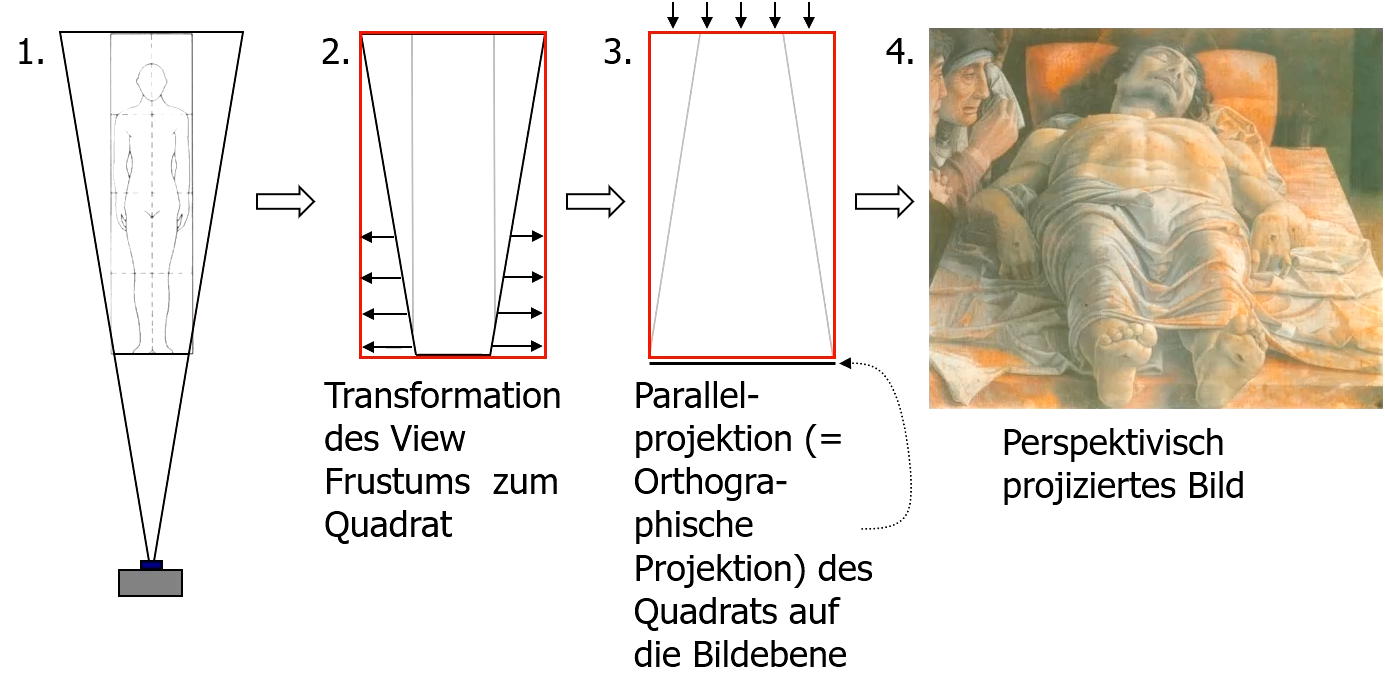
\includegraphics[width=400px]{images/perspektivischeProjektion.png}

\vspace{10px}

Betrachtet man Bilder von Kameras (oder das eigene Sichtbild, das auf die Netzhaut des Auges projiziert wird), so stellt man schnell fest, dass Dinge, die Nahe am Betrachter sind, größer sind, als Dinge, die weiter entfernt sind. Dieses Verhalten können wir auch bei der Projektion in der Computergraphik herstellen, um realistische Bilder zu erzeugen.\\
\begin{enumerate}
    \item Zunächst wird mithilfe des Kameramodells aus dem vorherigen Abschnitt der zu rendernde Bereich bestimmt. In der Realität wäre das der Bereich, dessen Lichtstrahlen durch ihre Position bedingt durch die Pupille auf die Netzhaut gelangen können (nur in der Realität ist der Bereich nicht nach vorne und hinten begrenzt). Das Bett, auf dem der Mensch auf dem Bild liegt bedeckt also den kompletten vorderen Rand des View Frustums und hinten ist neben dem Bett auch noch ein Stück der Umgebung im Bild.
    \item Nun wird der Pyramidenstumpf mittels einer Transformation so verzerrt, dass sich ein Quader (nicht Quadrat wie auf dem Bild steht!) bildet. Dadurch werden Objekte, die näher sind breiter. Auf diese Weise kann man sich auch leicht vorstellen, dass, wenn man den Öffnungswinkel der Kamera vergrößert, dieser Effekt stärker wird, d.h. weiter entfernte Objekte wirken dann noch kleiner und nähere noch größer. Auf unserem Bild wird das Bett an seiner vorderen Kante gestreckt, sodass seine eigentlich parallelen Seitenkanten auf dem Bild nach hinten spitz zusammenlaufen.
    \item Nun wird eine Parallelprojektion/orthographische Projektion durchgeführt, bei der der Quader auf ein Rechteck (das eigentliche Bild) abgebildet wird. Dabei ist es intuitiv notwendig, dass weiter vorne liegende Objekte weiter hinten liegende Objekte überlagern müssen.
\end{enumerate}

\subsubsection*{Projektionsmöglichkeiten}


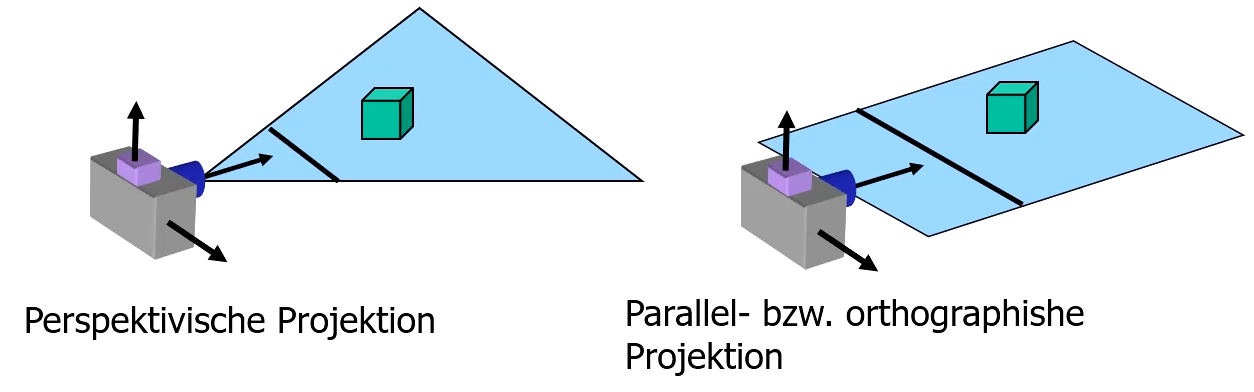
\includegraphics[width=300px]{images/projektionsmoeglichkeiten.png}


OpenGL biete neben der perspektivischen Projektion auch noch die Möglichkeit Parallelprojektion/orthographische Projektion zu benutzen. Diese Projektionsmethode haben wir bereits kennengelernt, als wir die perspektivische Projektion betrachtet haben, da sie immer notwendig ist, um den 3-dimensionalen Raum auf ein 2-dimensionales Bild zu projizieren. Benutzt man nur Parallelprojektion (d.h. nicht bloß im Rahmen der ''Toolchain''), dann ist eigentlich die Kamera, die auf dem Bild eingezeichnet ist, überflüssig. Alle Objekte werden dann direkt auf die schwarze Linie, die das Bild darstellen soll, abgebildet. In der Anwendung bedeutet das, dass die Perspektive alleine durch die Position und Größe der Clipping-Ebenen definiert ist und jedes Objekt unabhängig von seiner Position im Bild genau die größe hat, die es in der Realität hat (aber man kann das Bild danach natürlich noch skalieren). Das Größenverhältnis von Objekten bleibt auf dem Bild so, wie es in der Realität ist. Dieses Verhalten ist unnatürlich. Dabei entstehen Bilder, die ähnlich sind wie das folgende:

\vspace{10px}

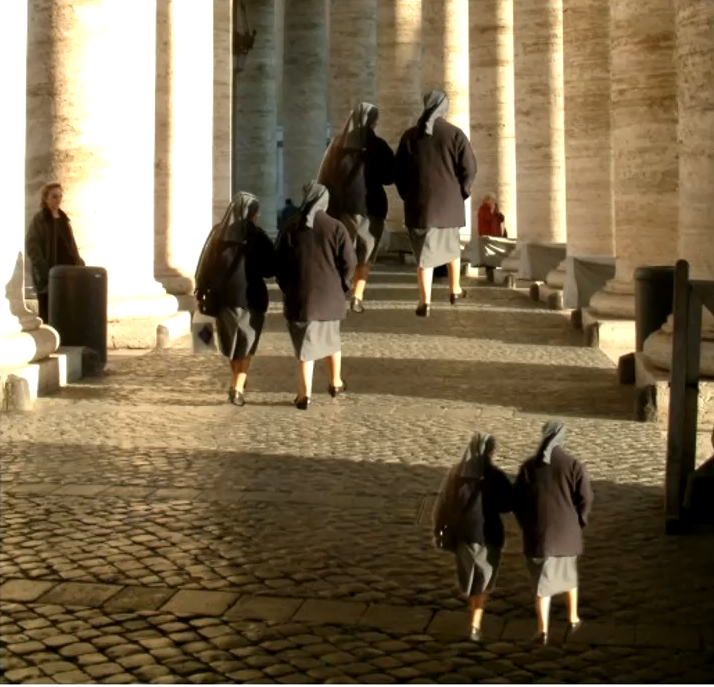
\includegraphics[width=300px]{images/perspektivischeWahrnehmung.png}

\subsection{Projektionsverfahren in OpenGL}
Die Projektionsmöglichkeiten werden in OpenGL auch über die Multiplikation der aktuellen Matrix mit Transformationsmatrizen geregelt. Dafür gibt es bestimmte Funktionen:

\subsubsection*{Orthographische Projektion}

\lstinputlisting[language=c++]{src/snippets/glOrtho.c++}

Der Funktionsaufruf erstellt eine Matrix für eine orthographische Projektion und multipliziert sie mit der aktuellen Matrix, indem er statt einem View Frustum einen View Quader definiert. Der ganze Inhalt des Quaders wird also auf die near Clipping Plane projiziert, welche dann auf das Ausgabefenster gemapt wird.

\begin{itemize}
    \item \textbf{left, bottom} geben den linken unteren Eckpunkt und \textbf{right, top} den rechten oberen Eckpunkt für die Clipping Planes an. Mittels der Information über die 2 Diagonalen Punkte und der Information, dass ein Rechteck entstehen soll, ist die größe des Rechtecks definiert
    \item \textbf{near} und \textbf{far} beschreiben die Entfernung zum Betrachter mit denen die zwei identisch großen Clipping Planes platziert werden sollen
    \item Die Clipping Planes werden so ausgerichtet, dass der Betrachter orthogonal auf sie schaut.
\end{itemize}

\subsubsection*{Perspektivische Projektion}

\lstinputlisting[]{src/snippets/gluPerspective.cpp}

Diese Funktion definiert ein View Frustum im Weltkoordinatensystem, generiert daraus eine Transformationsmatrix und multipliziert sie mit der aktuellen Matrix.

\begin{itemize}
    \item \textbf{fovy} gibt den Öffnungswinkel in y-Richtung an.
    \item \textbf{aspect} gibt das Seitenverhältnis $x \div y$ an.
    \item \textbf{zNear} bezeichnet die Distanz des Betrachters zur near-clipping-plane
    \item \textbf{zFar} bezeichnet die Distanz des Betrachters zur far-clipping-plane
\end{itemize}

Die konkreten Seitenlängen lassen sich für jeden Teil des Frustums also durch den Öffnungswinkel, die Entfernung, das Seitenverhältnis und den aktuellen Standpunkt des Beobachters (Standardmäßig im Ursprung, ansonsten mit \textit{gluLookAt} veränderbar) bestimmen. Somit ist das Frustum vollständig definiert.

\subsubsection*{Bewegung des Betrachters}

\lstinputlisting{src/snippets/gluLookAt.cpp}

Diese Funktion ermöglicht es den Betrachter zu verschieben und seine Ausrichtung zu verändern.\\
Wenn der Betrachter verschoben wird, \textbf{bewegen sich die Clipping-Planes mit ihm.}

\begin{itemize}
    \item \textbf{eyeX, eyeY, eyeZ} beschreiben den Ortsvektor der Linse des Betrachters
    \item \textbf{centerX, centerY, centerZ} beschreiben den Ortsvektor des Punktes auf die der Betrachter schaut
    \item \textbf{upX, upY, upZ} beschreibt den Ortsvektor des Punktes, der vom Betrachter aus als oben betrachtet wird
\end{itemize}

